\documentclass[a4paper,11pt,abstracton,hidelinks]{scrartcl}
\usepackage{dphil}
\addbibresource{refs.bib}
% hide section numbers
\setcounter{secnumdepth}{0}


\title{
Chapter 6. The evolution and spread of target-site resistance to pyrethroid insecticides
}


\author{}


\begin{document}
\renewcommand{\abstractname}{Summary}


\maketitle


%%%%%%%%%%%%%%%%%%%%%%%%%%%%%%%%%%%%%%%%%%%%%%%%%%%%%%%%%%%%%%%%%%%%%%%%%%%%%%%
%%%%%%%%%%%%%%%%%%%%%%%%%%%%%%%%%%%%%%%%%%%%%%%%%%%%%%%%%%%%%%%%%%%%%%%%%%%%%%%
%%%%%%%%%%%%%%%%%%%%%%%%%%%%%%%%%%%%%%%%%%%%%%%%%%%%%%%%%%%%%%%%%%%%%%%%%%%%%%%
\begin{abstract}


Resistance to pyrethroid insecticides is a serious challenge for malaria vector control in Africa, because pyrethroids remain a vital component of all long-lasting insecticidal bed-nets currently available for public health use.
%
Target-site resistance to pyrethroids involves nucleotide substitutions in the voltage-gated sodium channel gene (\textit{Vgsc}), which encodes an essential component of the insect nervous system and the binding target for pyrethroid molecules.
%
In this chapter, I use genome variation data from phase one of the Ag1000G project to study the molecular evolution and geographical spread of pyrethroid target-site resistance among nine mosquito populations.
%
I describe non-synonymous nucleotide variation throughout the entire gene coding sequence, including both known and novel polymorphisms, and report population allele frequencies and patterns of linkage disequilibrium.
%
I then analyse the genetic backgrounds on which resistance alleles are found, to look for evidence of the geographical spread of resistance via contemporary gene flow, and to confirm positive selection for resistance alleles.
%
I conclude by identifying a smaller subset of marker SNPs which could be used to track the further spread of resistance via low-cost high-throughput genetic assays.
%
These analyses show that the molecular basis of pyrethroid target-site resistance is substantially more complex and diverse than previously appreciated in these species, and demonstrate that long-distance gene flow between countries and adaptive introgression between species are both playing a major part in the rising prevalence of resistance alleles.


\end{abstract}


\tableofcontents


%%%%%%%%%%%%%%%%%%%%%%%%%%%%%%%%%%%%%%%%%%%%%%%%%%%%%%%%%%%%%%%%%%%%%%%%%%%%%%%
%%%%%%%%%%%%%%%%%%%%%%%%%%%%%%%%%%%%%%%%%%%%%%%%%%%%%%%%%%%%%%%%%%%%%%%%%%%%%%%
%%%%%%%%%%%%%%%%%%%%%%%%%%%%%%%%%%%%%%%%%%%%%%%%%%%%%%%%%%%%%%%%%%%%%%%%%%%%%%%
\section{Introduction}\label{sec:introduction}


%%%%%%%%%%%%%%%%%%%%%%%%%%%%%%%%%%%%%%%%%%%%%%%%%%%%%%%%%%%%%%%%%%%%%%%%%%%%%%%
%%%%%%%%%%%%%%%%%%%%%%%%%%%%%%%%%%%%%%%%%%%%%%%%%%%%%%%%%%%%%%%%%%%%%%%%%%%%%%%
\subsection{Pyrethroids in malaria vector control}\label{subsec:intro-pyrethroid-llins}


Pyrethroids are a class of synthetic insecticides, based on a natural compound pyrethrin found in the flowers of pyrethrum (Chrysanthemum) plants~\parencite{Elliott1989}.
%
Pyrethroids suitable for commercial use in agriculture and public health were discovered in the 1970s, and fall into two major groups based on chemical structure, either type I (e.g., permethrin~\parencite{Elliott1973}) or type II (e.g., deltamethrin~\parencite{Elliott1974}).
%
These compounds have a high toxicity to insects but relatively low toxicity to mammals, and are photostable but do not accumulate to contaminate the environment unlike insecticides used previously such as DDT or dieldrin.
%
Pyrethroids were approved for use in public health by the WHO pesticide evaluation scheme (WHOPES) in 1978~\parencite{Quelennec1988}.
%
Landmark studies during the 1980s and 1990s showed that the use of pyrethroid-treated bed-nets caused a significant reduction in malaria prevalence~\parencite{Carnevale2019}.
%
Advances in net manufacturing during that period allowed the development of long-lasting insecticidal nets (LLINs), which retain insecticidal activity for up to 3 years without re-treatment.
%
Pyrethroid LLINs have become the cornerstone of efforts to control malaria in Africa, with more than 100 million nets distributed in Africa each year since 2013~\parencite{Bhatt2015,AMP2020}.


%%%%%%%%%%%%%%%%%%%%%%%%%%%%%%%%%%%%%%%%%%%%%%%%%%%%%%%%%%%%%%%%%%%%%%%%%%%%%%%
%%%%%%%%%%%%%%%%%%%%%%%%%%%%%%%%%%%%%%%%%%%%%%%%%%%%%%%%%%%%%%%%%%%%%%%%%%%%%%%
\subsection{Pyrethroid resistance in the \textit{Anopheles gambiae} complex}\label{subsec:intro-pyrethroid-resistance}


The first reports of pyrethroid resistance in \agam\ originated from  C\^ote d'Ivoire~\parencite{Elissa1993} and Kenya~\parencite{Vulule1994}.
%
Subsequently, a study of six countries found pyrethroid resistance in Burkina Faso, C\^ote d'Ivoire and Benin~\parencite{Chandre1999}.
%
In parallel with the major scale-up of LLIN distributions from 2000 onwards, malaria control programmes have routinely performed bioassays to monitor pyrethroid resistance~\parencite{WHO2018TPIRM,WHO2017FNPMMIR}.
%
As those data have accumulated, it has become clear that both the prevalence and intensity of pyrethroid resistance have increased~\parencite{Ranson2011,Hemingway2016,WHO2012GPIRM,WHO2018GRIR,IIRC2018}.
%
Geostatistical modelling of bioassay data has supported this, showing a dramatic increase in the prevalence of resistance across sub-Saharan Africa over the period 2005--2017, although the picture remains complex, with considerable spatial heterogeneity~\parencite{Hancock2020}.


%%%%%%%%%%%%%%%%%%%%%%%%%%%%%%%%%%%%%%%%%%%%%%%%%%%%%%%%%%%%%%%%%%%%%%%%%%%%%%%
%%%%%%%%%%%%%%%%%%%%%%%%%%%%%%%%%%%%%%%%%%%%%%%%%%%%%%%%%%%%%%%%%%%%%%%%%%%%%%%
\subsection{The pyrethroid mode of action}\label{subsec:intro-moa}


Pyrethroid molecules interact with the voltage-gated sodium channel (VGSC), an essential membrane protein which propagates nerve impulses via action potentials~\parencite{Dong2014}.
%
In all insects, the VGSC protein comprises four homologous domains (I-IV), each of which has six transmembrane segments (S1-S6), which together form a gated pore that is sensitive to changes in membrane potential.
%
Under normal function, the channel opens during the rising phase of an action potential, allowing sodium ions to flow into the cell, then closes shortly afterwards, to allow re-polarisation of the membrane.
%
The structure of the protein creates some rotational symmetry, and it is believed that pyrethroids can bind to either of two analogous sites within the pore, referred to as PyR1 and PyR2~\parencite{Du2013}.
%
Pyrethroid binding alters gating behaviour, enhancing activation and inhibiting inactivation, causing the channel to remain open, which at the cellular level causes continuous firing of nerve impulses~\parencite{Dong2014}.
%
The VGSC protein of \agam\ comprises 2139 amino acids and has a high degree of homology with other insects, sharing the same overall topology~\parencite{Davies2007}.


%%%%%%%%%%%%%%%%%%%%%%%%%%%%%%%%%%%%%%%%%%%%%%%%%%%%%%%%%%%%%%%%%%%%%%%%%%%%%%%
%%%%%%%%%%%%%%%%%%%%%%%%%%%%%%%%%%%%%%%%%%%%%%%%%%%%%%%%%%%%%%%%%%%%%%%%%%%%%%%
\subsection{The molecular basis of pyrethroid target-site resistance in \agam}\label{subsec:intro-mol}


Any variations within the VGSC protein which alter the action of pyrethroids are known collectively as pyrethroid target-site resistance.
%
Prior to the present study, the molecular basis of pyrethroid target-site resistance in \agam\ appeared relatively straightforward.
%
An \texttt{L995F} substitution, initially found in West Africa~\parencite{MartinezTorres1998}, and an \texttt{L995S} substitution, initially found in East Africa~\parencite{Ranson2000a}, have both been shown to confer resistance to pyrethroids and DDT\footnotemark.
%
\footnotetext{Codon numbering is given relative to \agam\ transcript \texttt{AGAP004707-RA} in gene annotation set AgamP4.4. A mapping to \textit{D. melanogaster} codon numbers is given in~\ref{table:snps}.}
%
A third substitution, \texttt{N1570Y}, was subsequently found in West and Central Africa, occurring exclusively in combination with \texttt{L995F}~\parencite{Jones2012}.
%
\textit{In vitro}, VGSC double mutants carrying either \texttt{L995F} or \texttt{L995S} together with \texttt{N1570Y} are substantially more resistant to pyrethroids than \texttt{L995F} or \texttt{L995S} alone~\parencite{Wang2015}.
%
In other insects, the molecular basis of pyrethroid target-site resistance is more varied.
%
For example, in the invasive mosquito species \textit{Aedes aegypti}, 11 amino acid substitutions have been found in natural populations and associated with pyrethroid resistance~\parencite{Du2016,Haddi2017}.
%
Across all arthropods, more than 50 sodium channel SNPs or combinations of SNPs have been associated with pyrethroid resistance~\parencite{Dong2014}.
%
Since discovery of the \texttt{L995F} and \texttt{L995S} substitutions, studies in \agam\ have mostly focused on typing those polymorphisms, or sequencing a small region of the gene, and thus the full coding sequence has not been fully surveyed for variation in natural populations.


%%%%%%%%%%%%%%%%%%%%%%%%%%%%%%%%%%%%%%%%%%%%%%%%%%%%%%%%%%%%%%%%%%%%%%%%%%%%%%%
%%%%%%%%%%%%%%%%%%%%%%%%%%%%%%%%%%%%%%%%%%%%%%%%%%%%%%%%%%%%%%%%%%%%%%%%%%%%%%%
\subsection{The spread of pyrethroid target-site resistance in \agam\ and \acol}\label{subsec:intro-spread}


The \texttt{L995F} and \texttt{L995S} alleles have now been observed in multiple countries in both West and East Africa, with \texttt{L995F} being widespread particularly in West Africa~\parencite{WHO2018GRIR}.
%
These alleles have also been found in both \agam\ and \acol~\parencite{Clarkson2014,Norris2015,Djouaka2018}.
%
In West Africa, \texttt{L995F} has spread from \agam\ to \acol~\parencite{Clarkson2014,Norris2015}.
%
However, for each of these alleles, it is not clear whether it is spreading between countries via contemporary gene flow, or whether there are multiple geographical origins of resistance.
%
\textcite{Pinto2007} genotyped Vgsc codon 995 and performed partial sequencing of the upstream intron in \agam\ from 15 African countries, finding two common haplotypes carrying \texttt{L995F}, and a further two haplotypes associated with \texttt{L995S}.
%
Some of these haplotypes where shared between countries, but there were only four informative SNPs within the 438 bp region sequenced, and so resolution was not sufficient to infer gene flow with confidence.


%%%%%%%%%%%%%%%%%%%%%%%%%%%%%%%%%%%%%%%%%%%%%%%%%%%%%%%%%%%%%%%%%%%%%%%%%%%%%%%
%%%%%%%%%%%%%%%%%%%%%%%%%%%%%%%%%%%%%%%%%%%%%%%%%%%%%%%%%%%%%%%%%%%%%%%%%%%%%%%
\subsection{Scope of this chapter}\label{subsec:intro-scope}


In this chapter I analyse data from phase 1 of the Ag1000G project to investigate the molecular evolution and geographical spread of target-site resistance to pyrethroids.
%
I report non-synonymous SNPs within the \textit{Vgsc} gene that occur at appreciable frequency within one or more populations.
%
I also investigate the linkage between these SNPs, to determine whether some alleles occur in combination with others, and thus may have a synergistic effect.
%
I then use data on non-coding SNPs both within the gene introns and in the flanking intergenic sequences to investigate the haplotypes on which resistance alleles occur.
%
I use analyses of genetic relatedness between haplotypes to make inferences about gene flow events between populations from different geographical locations and species.
%
The work described in this chapter was performed as part of a broader collaboration within the Ag1000G Consortium analysing insecticide resistance genes, particularly with MalariaGEN Resource Center team colleague Chris Clarkson.
%
My contributions, described in this chapter, were to investigate the population-genetic aspects of resistance.
%
Any work carried out jointly is noted in the relevant section.


%%%%%%%%%%%%%%%%%%%%%%%%%%%%%%%%%%%%%%%%%%%%%%%%%%%%%%%%%%%%%%%%%%%%%%%%%%%%%%%
%%%%%%%%%%%%%%%%%%%%%%%%%%%%%%%%%%%%%%%%%%%%%%%%%%%%%%%%%%%%%%%%%%%%%%%%%%%%%%%
%%%%%%%%%%%%%%%%%%%%%%%%%%%%%%%%%%%%%%%%%%%%%%%%%%%%%%%%%%%%%%%%%%%%%%%%%%%%%%%
\section{Results}\label{sec:results}


%%%%%%%%%%%%%%%%%%%%%%%%%%%%%%%%%%%%%%%%%%%%%%%%%%%%%%%%%%%%%%%%%%%%%%%%%%%%%%%
%%%%%%%%%%%%%%%%%%%%%%%%%%%%%%%%%%%%%%%%%%%%%%%%%%%%%%%%%%%%%%%%%%%%%%%%%%%%%%%
\subsection{Non-synonymous SNPs within the \textit{Vgsc} gene}\label{subsec:results-snps}


There were 63 non-synonymous SNPs within the \textit{Vgsc} gene (\texttt{AGAP004707}) that were polymorphic within the Ag1000G phase 1 dataset.
%
For these SNPs, I computed the frequency of each non-synonymous variant allele within each of nine populations defined by species and country of origin.
%
If an allele has a resistance phenotype and has been under positive selection, then it will occur at some appreciable frequency in one or more populations.
%
I therefore filtered the SNPs to remove any rare variants, retaining only those SNPs with a variant allele occurring at a frequency above 4\% in at least one population.
%
This resulted in a set of 21 SNPs, including two multiallelic SNPs (Table~\ref{table:snps}).


%% Table 1 - Functional SNPs.
%
\afterpage{%
\begin{landscape}
\thispagestyle{empty}
\begin{table}[h]
  \scriptsize
  \centering
  \begin{threeparttable}

  \caption{
%
\textbf{Non-synonymous SNPs in the \textit{Vgsc} gene}.
%
AO=Angola; BF=Burkina Faso; GN=Guinea; CM=Cameroon; GA=Gabon; UG=Uganda; KE=Kenya; GW=Guinea-Bissau; \textit{Ac}=\textit{An. coluzzii}; \textit{Ag}=\textit{An. gambiae}.
%
Species status of specimens from Kenya and Guinea-Bissau is uncertain.
%
All variants are at 4\% frequency or above in one or more of the 9 Ag1000G phase 1 populations, with the exception of \texttt{2,400,071 G>T} which is only found in the CM\emph{Ag} population at 0.4\% frequency but is included because another mutation (\texttt{2,400,071 G>A}) is found at the same position causing the same amino acid substitution (\texttt{M490I}).
}

  \label{table:snps}

  
\begin{tabular}{lllrrrrrrrrr}
\toprule
\multicolumn{3}{c}{Variant} &
\multicolumn{9}{c}{Population allele frequency (\%)}\\
\cmidrule(r){1-3}
\cmidrule(r){4-12}
Position\tnote{1} & 
\emph{Ag}\tnote{2} & 
\emph{Md}\tnote{3} &
AO\emph{Ac} &
BF\emph{Ac} & 
GN\emph{Ag} & 
BF\emph{Ag} & 
CM\emph{Ag} & 
GA\emph{Ag} & 
UG\emph{Ag} & 
KE & 
GW\\
\midrule

\texttt{2,390,177 G>A} & \texttt{R254K} & \texttt{R261} & 0 & 0 & 0 & 0 & 32 & 21 & 0 & 0 & 0 \\

\texttt{2,391,228 G>C} & \texttt{V402L} & \texttt{V410} & 0 & 7 & 0 & 0 & 0 & 0 & 0 & 0 & 0 \\

\texttt{2,391,228 G>T} & \texttt{V402L} & \texttt{V410} & 0 & 7 & 0 & 0 & 0 & 0 & 0 & 0 & 0 \\

\texttt{2,399,997 G>C} & \texttt{D466H} & \texttt{-} & 0 & 0 & 0 & 0 & 7 & 0 & 0 & 0 & 0 \\

\texttt{2,400,071 G>A} & \texttt{M490I} & \texttt{M508} & 0 & 0 & 0 & 0 & 0 & 0 & 0 & 18 & 0 \\

\texttt{2,400,071 G>T} & \texttt{M490I} & \texttt{M508} & 0 & 0 & 0 & 0 & 0 & 0 & 0 & 0 & 0 \\

\texttt{2,416,980 C>T} & \texttt{T791M} & \texttt{T810} & 0 & 1 & 13 & 14 & 0 & 0 & 0 & 0 & 0 \\

\texttt{2,422,651 T>C} & \texttt{L995S} & \texttt{L1014} & 0 & 0 & 0 & 0 & 15 & 64 & 100 & 76 & 0 \\

\texttt{2,422,652 A>T} & \texttt{L995F} & \texttt{L1014} & 86 & 85 & 100 & 100 & 53 & 36 & 0 & 0 & 0 \\

\texttt{2,424,384 C>T} & \texttt{A1125V} & \texttt{K1133} & 9 & 0 & 0 & 0 & 0 & 0 & 0 & 0 & 0 \\

\texttt{2,425,077 G>A} & \texttt{V1254I} & \texttt{I1262} & 0 & 0 & 0 & 0 & 0 & 0 & 0 & 0 & 5 \\

\texttt{2,429,617 T>C} & \texttt{I1527T} & \texttt{I1532} & 0 & 14 & 0 & 0 & 0 & 0 & 0 & 0 & 0 \\

\texttt{2,429,745 A>T} & \texttt{N1570Y} & \texttt{N1575} & 0 & 26 & 10 & 22 & 6 & 0 & 0 & 0 & 0 \\

\texttt{2,429,897 A>G} & \texttt{E1597G} & \texttt{E1602} & 0 & 0 & 6 & 4 & 0 & 0 & 0 & 0 & 0 \\

\texttt{2,429,915 A>C} & \texttt{K1603T} & \texttt{K1608} & 0 & 5 & 0 & 0 & 0 & 0 & 0 & 0 & 0 \\

\texttt{2,430,424 G>T} & \texttt{A1746S} & \texttt{A1751} & 0 & 0 & 11 & 13 & 0 & 0 & 0 & 0 & 0 \\

\texttt{2,430,817 G>A} & \texttt{V1853I} & \texttt{V1858} & 0 & 0 & 8 & 5 & 0 & 0 & 0 & 0 & 0 \\

\texttt{2,430,863 T>C} & \texttt{I1868T} & \texttt{I1873} & 0 & 0 & 18 & 25 & 0 & 0 & 0 & 0 & 0 \\

\texttt{2,430,880 C>T} & \texttt{P1874S} & \texttt{P1879} & 0 & 21 & 0 & 0 & 0 & 0 & 0 & 0 & 0 \\

\texttt{2,430,881 C>T} & \texttt{P1874L} & \texttt{P1879} & 0 & 7 & 45 & 26 & 0 & 0 & 0 & 0 & 0 \\

\texttt{2,431,019 T>C} & \texttt{F1920S} & \texttt{Y1925} & 0 & 0 & 0 & 0 & 1 & 4 & 0 & 0 & 0 \\

\texttt{2,431,061 C>T} & \texttt{A1934V} & \texttt{A1939} & 0 & 12 & 0 & 0 & 0 & 0 & 0 & 0 & 0 \\

\texttt{2,431,079 T>C} & \texttt{I1940T} & \texttt{I1945} & 0 & 4 & 0 & 0 & 7 & 0 & 0 & 0 & 0 \\

\bottomrule
\end{tabular}


  \begin{tablenotes}
    \footnotesize

    \item[1] Position relative to the AgamP3 reference sequence, chromosome arm 2L.

    \item[2] Codon numbering according to \emph{Anopheles gambiae} transcript AGAP004707-RA in gene annotations AgamP4.4.

    \item[3] Codon numbering according to \emph{Musca domestica} EMBL accession X96668.

  \end{tablenotes}

  \end{threeparttable}

\end{table}
\end{landscape}
\restoregeometry
} % end afterpage
%% end Table 1


The two known pyrethroid resistance variants in codon 995 were at the highest overall frequency in the cohort.
%
\texttt{L995F} was at high frequency in both \acol\ populations, at fixation in both West African \agam\ populations, and also present in the two central African \agam\ populations.
%
\texttt{L995S} was at high frequency in the Kenyan population, fixed in the Uganda \agam\ population, and also present in both central African \agam\ populations.
%
The combined frequency of \texttt{L995F} and \texttt{L995S} mutations in countries where both variants co-occurred was 68\% in Cameroon and 100\% in Gabon.
%
The other SNP with a known resistance phenotype in \agam, \texttt{N1570Y}, was present in \agam\ samples from Guinea and Cameroon and both species from Burkina Faso.


None of the remaining SNPs have a known phenotype in \agam\ or \acol.
%
Among these, the following SNPs are of particular interest, based on observations in other studies:
%
\begin{itemize}
    %
    \item \texttt{P1874L/S} - \texttt{P1874L} was the most common allele after the known resistance alleles, being found at 45\% and 26\% frequency in \agam\ from Burkina Faso and Cameroon respectively.
    %
    Both \texttt{P1874L} and \texttt{P1874S} were present in \acol\ from Burkina Faso, and the combined allele frequency of codon 1874 variants was 28\%.
    %
    \texttt{P1874L} was also present in sequencing data reported by \textcite{Jones2012} in samples of both \agam\ and \acol\ from Burkina Faso.
    %
    \texttt{P1874S} has not been reported elsewhere in mosquitoes, but was found in pyrethroid-resistant field strains of the diamond-back moth \textit{Plutella xylostella}~\parencite{Sonoda2010}.
    %
    \item \texttt{I1527T} - Previously reported by \textcite{Jones2012} at low frequency in \acol\ from Burkina Faso, this allele was at 14\% frequency in the Ag1000G \acol\ from Burkina Faso.
    %
    Recently, \textcite{Collins2019} reported \texttt{I1527T} in \agam\ from Guinea and found it was associated with resistance to permethrin.
    %
    \texttt{I1527T} has also been recently found in \textit{Aedes albopictus}~\parencite{Auteri2018}.
    %
    \item \texttt{V402L} - The SNP at \texttt{2L:2,391,228} had two variant alleles which both conferred \texttt{V402L}, and which were each at 7\% frequency in Burkina Faso \acol, but not found elsewhere.
    %
    Mutations in codon 410 have been shown to cause pyrethroid resistance in multiple insect species, and the pyrethroid resistance phenotype has also been confirmed and characterized in vitro~\parencite{Dong2014}.
    %
    Recently, \texttt{V402L} has been found in \textit{Aedes aegypti} where it confers high levels of resistance both type I and type II pyrethroids~\parencite{Haddi2017,VillanuevaSegura2020}.
    %
\end{itemize}
%


%%%%%%%%%%%%%%%%%%%%%%%%%%%%%%%%%%%%%%%%%%%%%%%%%%%%%%%%%%%%%%%%%%%%%%%%%%%%%%%
%%%%%%%%%%%%%%%%%%%%%%%%%%%%%%%%%%%%%%%%%%%%%%%%%%%%%%%%%%%%%%%%%%%%%%%%%%%%%%%
\subsection{Associations between non-synonymous SNPs}\label{subsec:results-ld}


In several insect species, two or more non-synonymous variants in the \textit{Vgsc} gene have been observed occurring together on the same haplotype.
%
For example, \texttt{N1570Y} is only found in \agam\ in combination with \texttt{L995F}~\parencite{Jones2012}.
%
Similarly, in the German cockroach \textit{Blatella germanica}, the combinations \texttt{L993F+E434K}, \texttt{L993F+C764R} and \texttt{L993F+E434K+C764R} have been found~\parencite{Tan2002}.
%
In the diamond back moth, the alleles \texttt{A1101T+P1879S} are found in combination~\parencite{Sonoda2010}.
%
In \textit{Aedes aegypti}, the combination \texttt{V410L+F1534C} has been observed~\parencite{Haddi2017}, as well as each allele separately.
%
The occurrence of alleles in combination is interesting because these alleles may act synergistically to enhance a pyrethroid resistance phenotype.
%
For example, the \texttt{L995F+N1570Y} combination is approximately ten times more resistant to permethrin than \texttt{L995F} alone~\parencite{Wang2015}.
%
Similarly, in the German cockroach, \texttt{L993F+E434K} and \texttt{L993F+C764R} are each approximately 20 times more resistant to deltamethrin than \texttt{L993F} alone~\parencite{Tan2002}, and the triple mutant \texttt{L993F+E434K+C764R} is 100 times more resistant.


To investigate associations between non-synonymous variants within the Ag1000G phase 1 dataset, I calculated the $D'$ linkage disequilibrium (LD) statistic between all pairs of variant alleles~\parencite{Lewontin1964}.
%
I then combined these data with allele frequencies, to identify three possible types of association:
%
\begin{itemize}
    %
    \item \textbf{Complete association} - Two alleles are only ever found in combination ($D' \approx 1$, equal allele frequencies).
    %
    \item \textbf{Subordinate association} - A primary allele, sometimes found alone, and a secondary allele, only ever found in combination with the primary allele ($D' \approx 1$, with one allele at higher frequency than the other).
    %
    \item \textbf{Partial association} - Two alleles, each observed alone and in combination ($-1 < D' < 1$).
    %
\end{itemize}


The computed LD values are shown together with overall allele frequencies within the Ag1000G phase 1 cohort in Fig.~\ref{fig:ld}.
%
Fourteen variant alleles were in subordinate association with \texttt{L995F} ($D' > 0.91$) including \texttt{N1570Y}, \texttt{P1874S} and \texttt{P1874L}.
%
There were also two triple-mutant combinations, \texttt{L995F+D466H+I1940T} and \texttt{L995F+T791M+A1746S}.
%
In contrast, there were no non-synonymous variant alleles in any kind of association with \texttt{L995S}.
%
Thus, substantial molecular evolution appears to be occurring on haplotype backgrounds carrying \texttt{L995F}.
%
Each of the two \texttt{V402L} alleles was in subordinate association with \texttt{I1527T}, but at the amino acid level, \texttt{V402L} and \texttt{I1527T} were in near-complete association, indicating a strong mutual dependence between them.


\begin{figure}[t!]
\centering
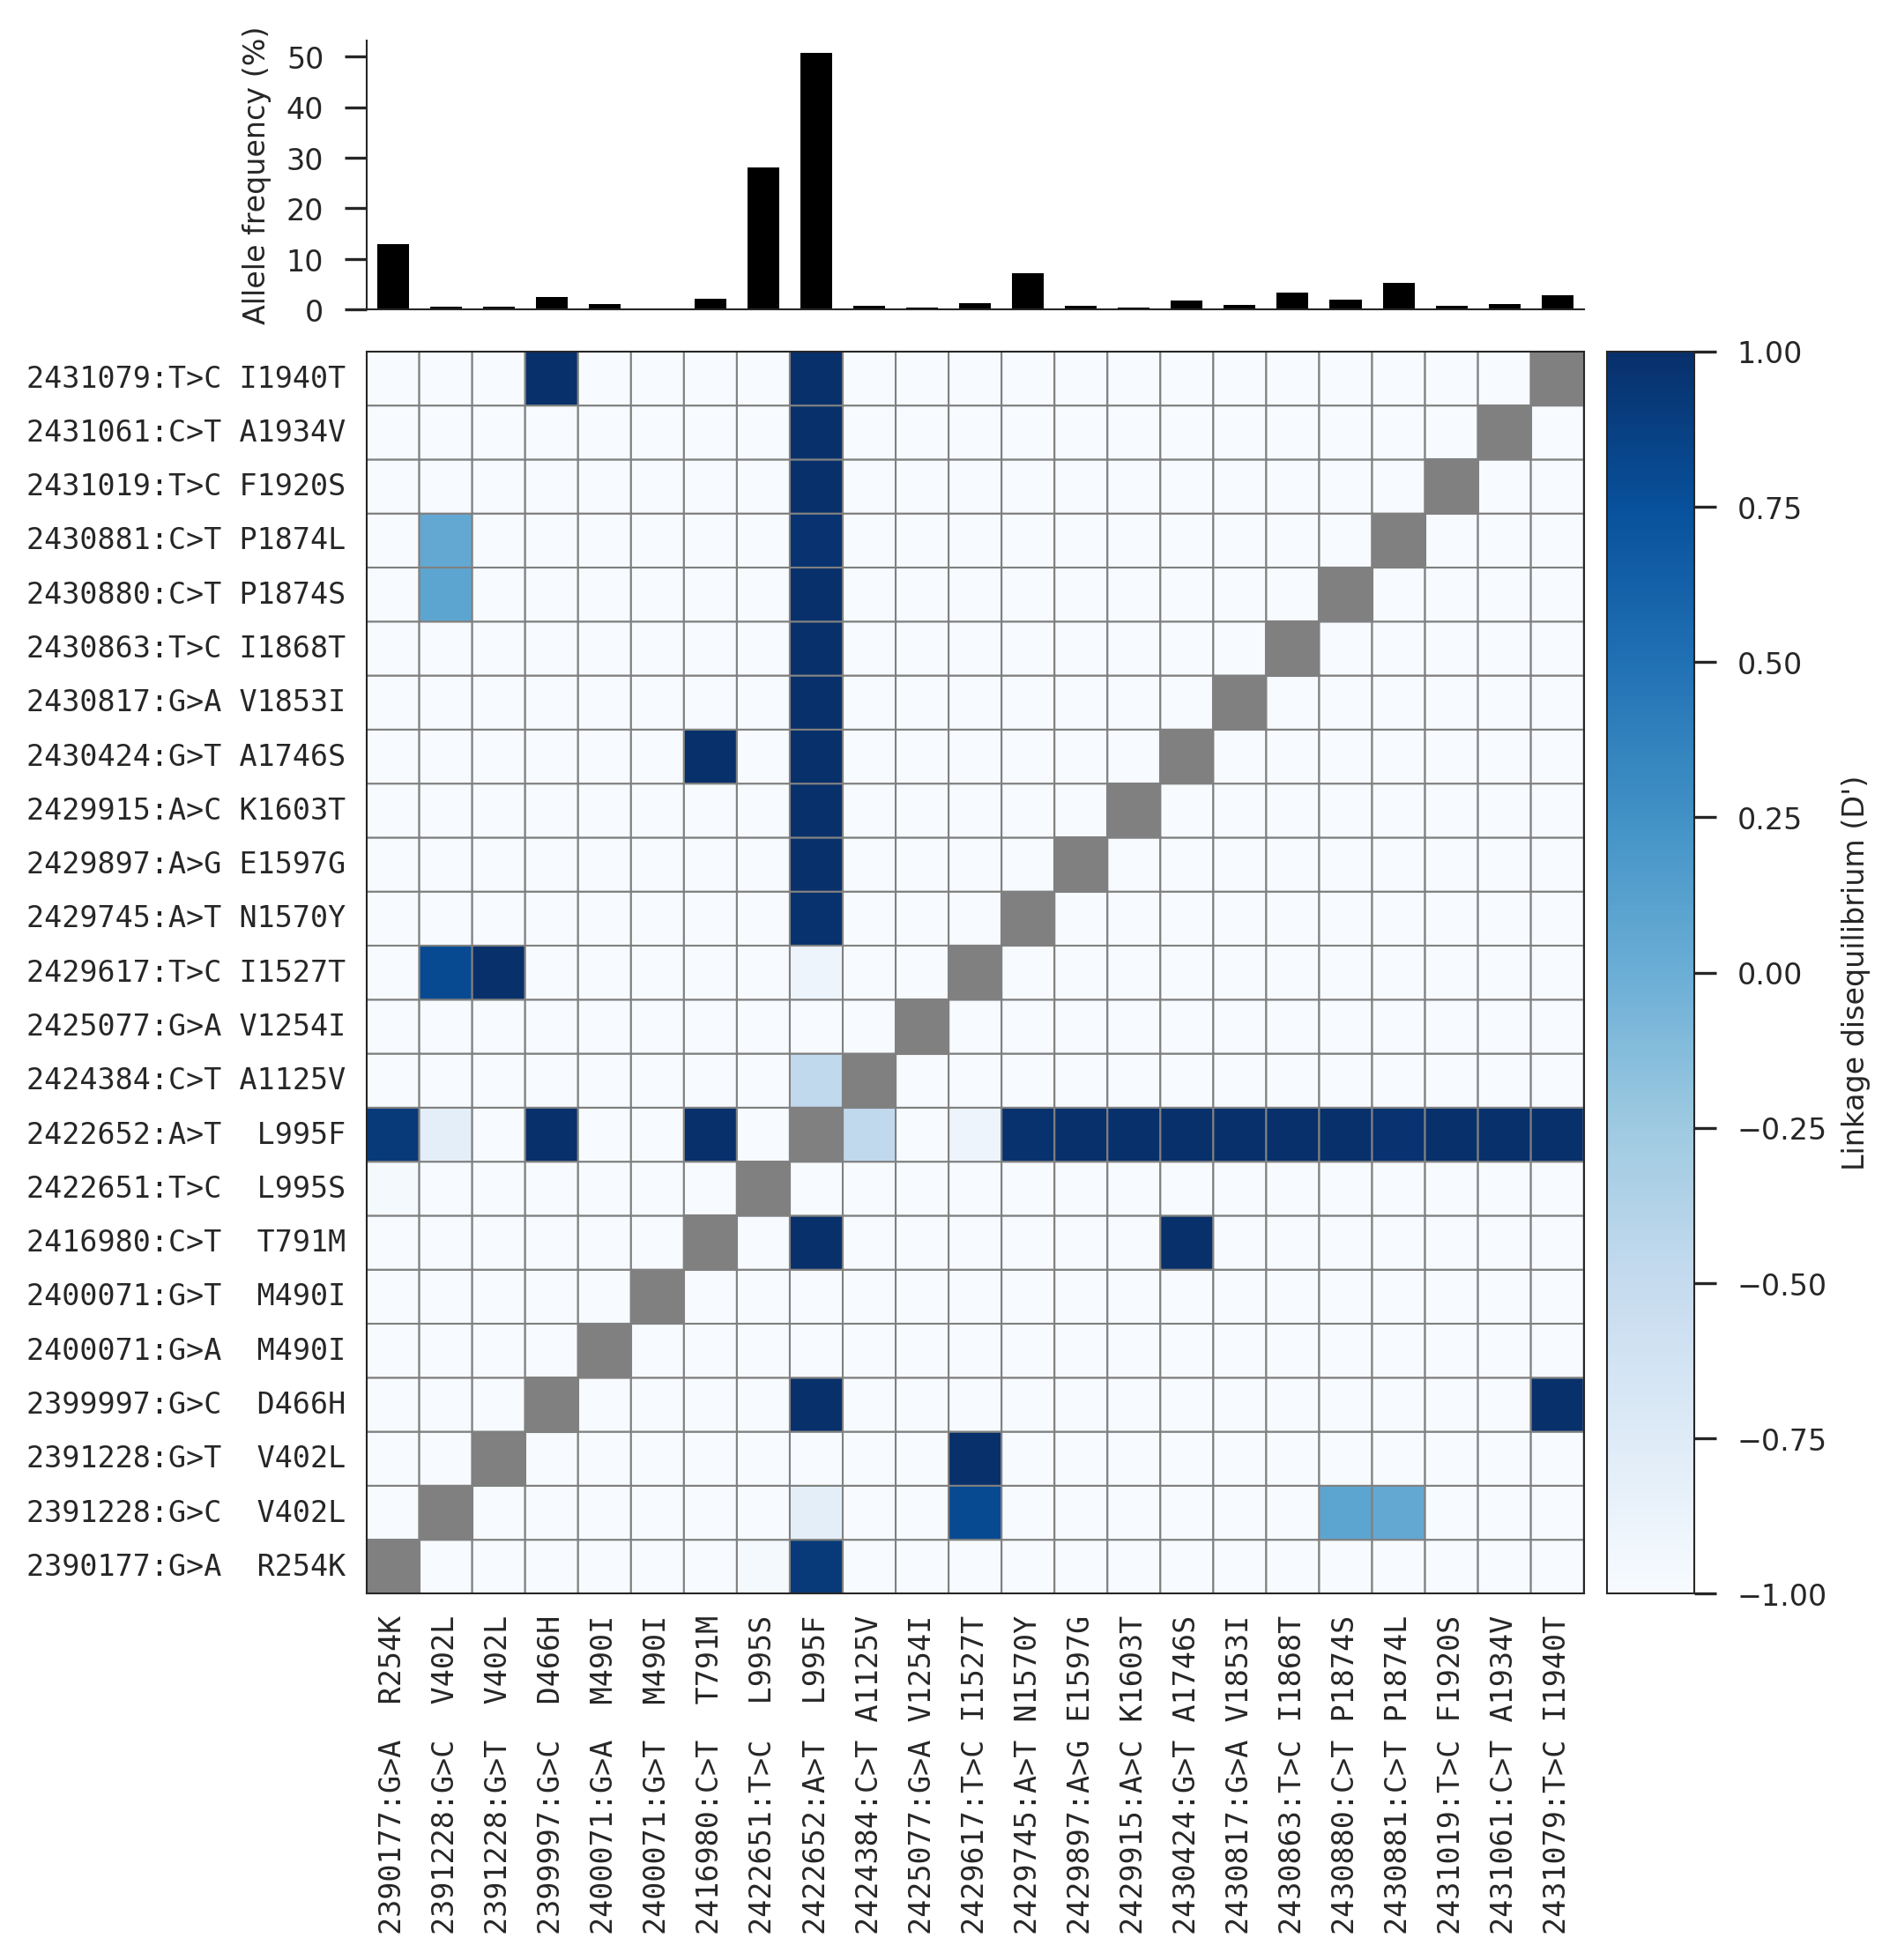
\includegraphics[width=0.9\linewidth,center]{artwork/chapter6/ld.png}
\caption{Linkage disequilibrium ($D'$) between non-synonymous variant alleles.
%
A value of 1 indicates that two alleles are in perfect linkage, meaning that one of the alleles is only ever found in combination with the other.
%
Conversely, a value of −1 indicates that two alleles are never found in combination with each other.
%
The bar plot at the top shows the frequency of each allele within the Ag1000G phase 1 cohort.
%
See Table~\ref{table:snps} for population allele frequencies.
}
\label{fig:ld}
\end{figure}


%%%%%%%%%%%%%%%%%%%%%%%%%%%%%%%%%%%%%%%%%%%%%%%%%%%%%%%%%%%%%%%%%%%%%%%%%%%%%%%
%%%%%%%%%%%%%%%%%%%%%%%%%%%%%%%%%%%%%%%%%%%%%%%%%%%%%%%%%%%%%%%%%%%%%%%%%%%%%%%
\subsection{Geographical spread of pyrethroid resistance alleles}\label{subsec:results-spread}


\begin{figure}[t!]
\centering
\begin{subfigure}[t]{1\textwidth}
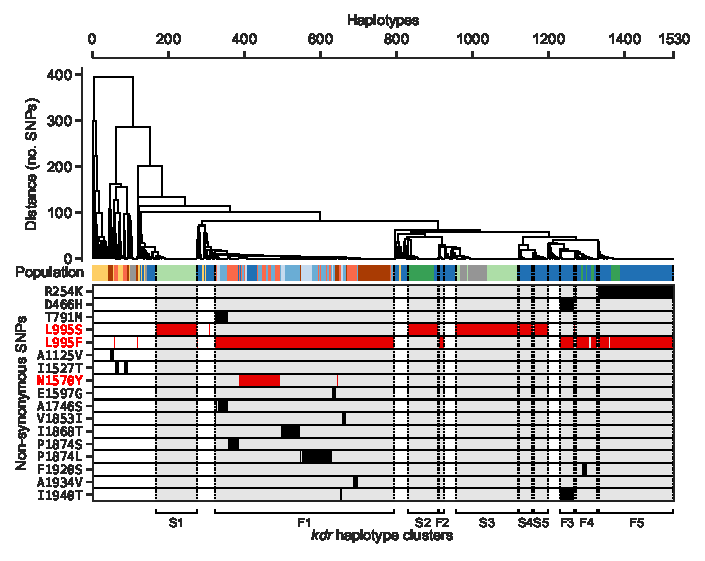
\includegraphics[width=1\linewidth,center]{artwork/chapter6/hapclust.pdf}
\end{subfigure}
\begin{subfigure}[t]{1\textwidth}
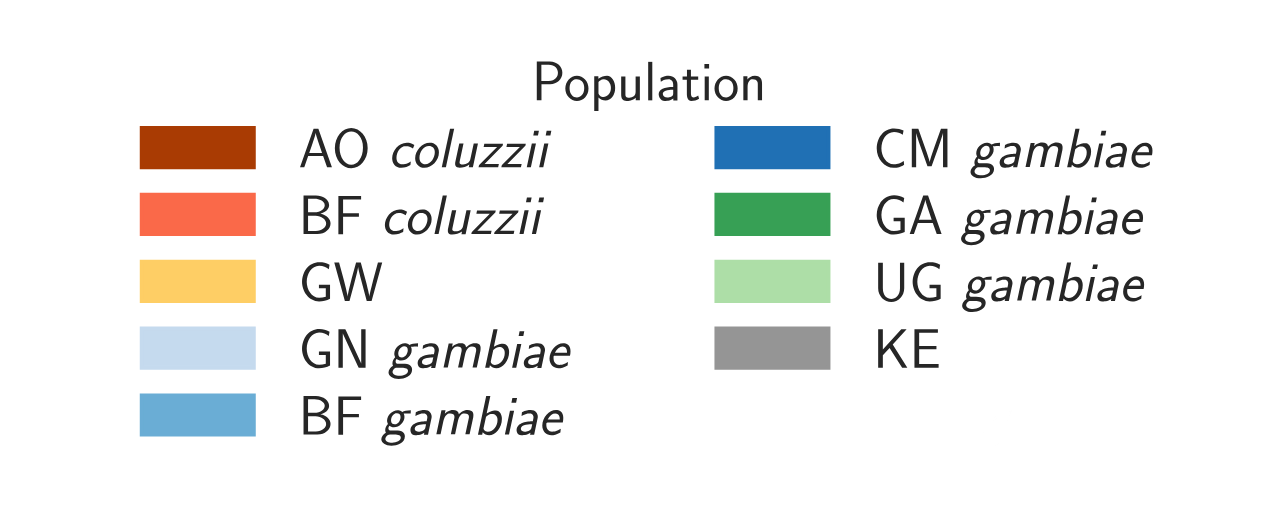
\includegraphics[width=.5\linewidth,center]{artwork/chapter6/pop_legend.png}
\end{subfigure}
\caption{Clustering of haplotypes within the \textit{Vgsc} gene.
The upper panel shows a dendrogram obtained by hierarchical clustering of haplotypes from wild-caught individuals.
%
The colour bar below shows the population of origin for each haplotype.
%
The lower panel shows alleles carried by each haplotype at non-synonymous SNPs (white=reference allele, black=alternate allele, red=previously known resistance allele).
%
At the lower margin, F1--F5 label clusters carrying the \texttt{L995F} allele, and S1--S5 label clusters carrying the \texttt{L995S} allele.
}
\label{fig:hapclust}
\end{figure}


To investigate evidence for geographical spread of pyrethroid resistance alleles, I analysed patterns of genetic similarity between the 1530 haplotypes in the Ag1000G phase 1 dataset.
%
The Ag1000G haplotypes were phased across the whole genome, and incorporate data on non-synonymous SNPs, both within the \textit{Vgsc} introns and in the flanking intergenic regions, which provide high resolution to identify different degrees of similarity between haplotypes.
%
I firstly analysed the region spanning the \textit{Vgsc} gene itself, which spans 73.5 kb and contains a total of 1,710 biallelic SNPs (1,607 intronic, 103 exonic) phased in the Ag1000G dataset.
%
I performed a hierarchical clustering of these haplotypes, based on the number of SNP differences between them, and constructed a dendrogram, shown in Fig.~\ref{fig:hapclust}.
%
The likely presence of recombination events within the genomic interval bounded by the \textit{Vgsc} gene, and the use of a simple distance metric and clustering method, means that this dendrogram cannot be interpreted as a complete phylogeny.
%
However, there were some clear patterns within these data.
%
In particular, there were several large clusters of near-identical haplotypes, each of which was strongly associated with either \texttt{L995F} or \texttt{L995S}.
%
To provide a means of navigating these data, I cut the dendrogram at a maximum distance of 12 SNPs.
%
I then labelled the five largest clusters containing the \texttt{L995F} allele as F1-F5, and the five largest clusters containing the \texttt{L995S} allele as S1-S5.
%
The clusters F1-F5 together accounted for 96\% of haplotypes carrying the \texttt{L995F} allele, and the clusters S1-S5 together accounted for 99\% of haplotypes carrying the \texttt{L995S} allele.


Five of these haplotype clusters carrying resistance alleles contained haplotypes from different countries and/or species.
%
Cluster F1 contained haplotypes from Burkina Faso, Guinea, Cameroon and Angola, and from both \agam\ and \acol.
%
Clusters F4, F5 and S2 each contained haplotypes from both Cameroon and Gabon \agam.
%
Cluster S3 contained haplotypes from both Uganda \agam\ and Kenya.
%
To confirm that this degree of haplotype similarity between different populations is unusual, and likely represents the result of contemporary gene flow driven by selection for resistance alleles in the \textit{Vgsc} gene, I analysed patterns of haplotype sharing between populations across the whole of chromosome arm 2L (Fig.~\ref{fig:xphh}).
%
For all pairs of populations which were both found within the same \textit{Vgsc} haplotype cluster, I also observed a clear signal of between-population haplotype homozygosity at the \textit{Vgsc} gene, which was not present elsewhere on the chromosome arm.
%
Conversely, for pairs of populations never found in the same \textit{Vgsc} haplotype cluster, levels of between-population haplotype homozygosity were similarly low across the whole chromosome arm.
%
Taken together, these results provide strong support for adaptive gene flow of pyrethroid resistance alleles between countries and species, in some cases separated by large geographical distances.


%%%%%%%%%%%%%%%%%%%%%%%%%%%%%%%%%%%%%%%%%%%%%%%%%%%%%%%%%%%%%%%%%%%%%%%%%%%%%%%
%%%%%%%%%%%%%%%%%%%%%%%%%%%%%%%%%%%%%%%%%%%%%%%%%%%%%%%%%%%%%%%%%%%%%%%%%%%%%%%
\subsection{Positive selection for pyrethroid resistance alleles}\label{subsec:results-selection}


To investigate evidence for positive selection on non-synonymous alleles, I performed an analysis of extended haplotype homozygosity (EHH)~\parencite{Sabeti2002}.
%
Haplotypes under recent positive selection will have increased rapidly in frequency, thus have had less time to be broken down by recombination, and should on average have longer regions of haplotype homozygosity relative to haplotypes carrying wild-type alleles.
%
I defined a core region spanning \textit{Vgsc} codon 995, and an additional 6 kb of flanking sequence, which was the minimum required to find core haplotypes corresponding to the haplotype clusters F1-F5 and S1-S5 identified via the clustering analysis described above.
%
I found 18 distinct haplotypes within this core region that were at a frequency above 1\% within the cohort.
%
These included core haplotypes corresponding to each of the 10 haplotype clusters carrying \texttt{L995F} or \texttt{L995S} alleles, as well as a core haplotype carrying \texttt{I1527T} which I labelled as L1 (due to it carrying the wild-type leucine at codon 995).
%
I also found a core haplotype corresponding to a group of haplotypes from Kenya carrying a \texttt{M490I} substitution, which I labelled L2.
%
All the other core haplotypes were labelled as wild-type (wt).
%
I then computed EHH decay for each core haplotype up to 1 Mb upstream and downstream of the core locus (Fig.~\ref{fig:ehh}).


\begin{figure}[t!]
\centering
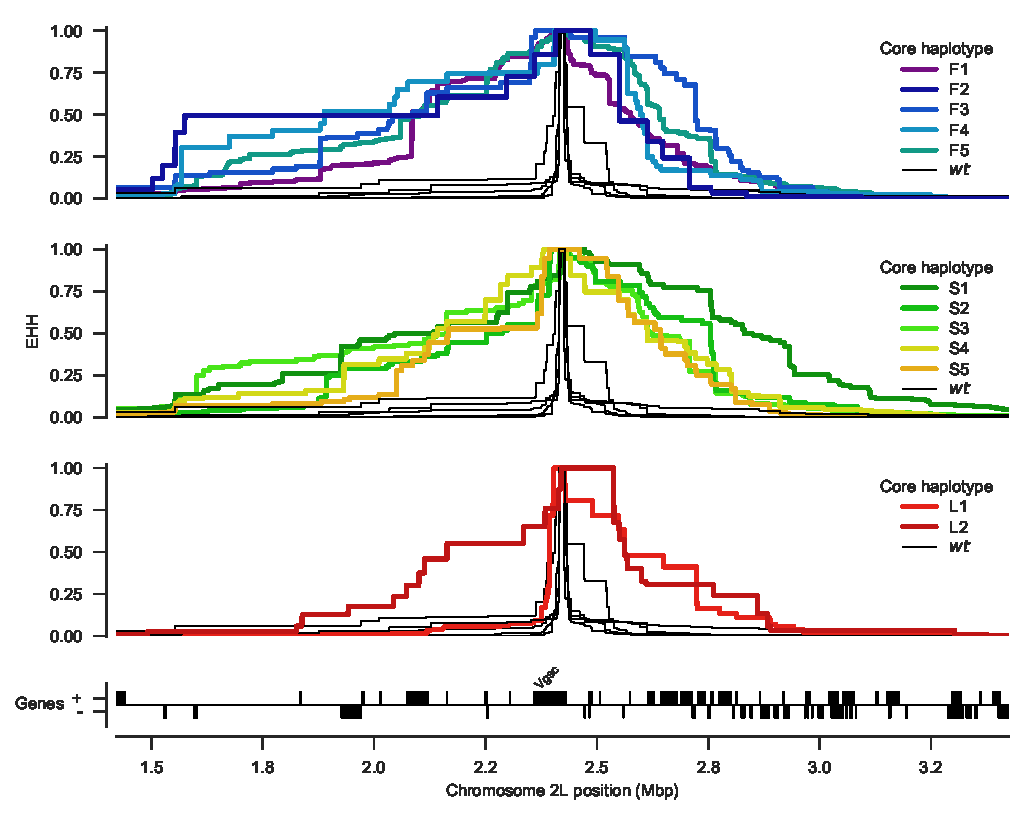
\includegraphics[width=1\linewidth,center]{artwork/chapter6/ehh.pdf}
\caption{Evidence for positive selection on haplotypes carrying known or putative resistance alleles.
%
Each panel plots the decay of extended haplotype homozygosity (EHH) for a set of core haplotypes centred on \textit{Vgsc} codon 995.
%
Core haplotypes F1--F5 carry the \texttt{L995F} allele, S1--S5 carry the \texttt{L995S} allele, L1 carries the \texttt{I1527T} allele, L2 carries the \texttt{M490I} allele.
%
Wild-type (wt) haplotypes do not carry known or putative resistance alleles.
%
A slower decay of EHH relative to wild-type haplotypes implies positive selection (each panel plots the same collection of wild-type haplotypes).
}
\label{fig:ehh}
\end{figure}


Haplotypes carrying either \texttt{L995F} or \texttt{L995S} all experienced slower decay of EHH relative to wild-type haplotypes, indicating positive selection for these resistance alleles.
%
Previous studies have reported evidence for different rates of EHH decay between \texttt{L995F} and \texttt{L995S} haplotypes, suggesting a difference in the timing and/or strength of selection.
%
I found no systematic difference in the extent of haplotype homozygosity when comparing F1-F5 (carrying \texttt{L995F}) against S1-S5 (carrying \texttt{L995S}) (Fig.~\ref{fig:pspd}).
%
There were, however, some differences between core haplotypes carrying the same allele.
%
For example, haplotypes were significantly longer for S1 (median 1.091 cM, 95\% bootstrap CI [1.076 - 1.091]) versus other core haplotypes carrying \texttt{L995S} (e.g., S2 median 0.699 cM, 95\% bootstrap CI [0.696 - 0.705]).
%
Longer shared haplotypes indicate a more recent common ancestor, and thus some of these core haplotypes may have experienced more recent and/or more intense selection than others.


The L1 haplotypes carrying \texttt{I1527T+V402L} exhibited a slow decay of EHH on the downstream flank of the gene, similar to haplotypes carrying \texttt{L995F} or \texttt{L995S}, indicating that this combination of alleles has experienced positive selection.
%
EHH decay on the upstream flank was faster, similar to wild-type haplotypes, but there were two separate SNPs conferring \texttt{V402L} within this group of haplotypes, and a faster EHH decay on this flank is consistent with recombination events bringing \texttt{V402L} alleles from different genetic backgrounds together with a haplotype carrying \texttt{I1527T}.
%
The L2 haplotype carrying \texttt{M490I} exhibited EHH decay on both flanks comparable to haplotypes carrying known resistance alleles.
%
This could indicate positive selection on the \texttt{M490I} allele, but these haplotypes are derived from a Kenyan mosquito population where there is evidence for a severe recent bottleneck as described in Chapter 4.
%
There were not enough wild-type haplotypes from Kenya with which to compare, thus this signal could also be due to the extreme demographic history of this population.


%%%%%%%%%%%%%%%%%%%%%%%%%%%%%%%%%%%%%%%%%%%%%%%%%%%%%%%%%%%%%%%%%%%%%%%%%%%%%%%
%%%%%%%%%%%%%%%%%%%%%%%%%%%%%%%%%%%%%%%%%%%%%%%%%%%%%%%%%%%%%%%%%%%%%%%%%%%%%%%
\subsection{Genetic surveillance of pyrethroid resistance}\label{subsec:results-tracking}


Entomological monitoring programmes supporting malaria vector control in Africa do in some cases genotype mosquitoes for known resistance alleles in \textit{Vgsc} codon 995, and use those results as an indicator for the presence of pyrethroid resistance, alongside results from resistance bioassays.
%
They typically do not, however, sequence the gene or genotype any other polymorphisms within the gene.
%
Thus, if there are other polymorphisms within the gene that cause or enhance pyrethroid resistance, these will not be detected.
%
Also, if a codon 995 resistance allele is observed, there is no way to know whether the allele is on a genetic background that has also been observed in other mosquito populations, and thus whether resistance alleles are emerging locally or spreading from elsewhere.
%
Whole-genome sequencing (WGS) of individual mosquitoes clearly provides data of sufficient resolution to answer these questions, and could be used to provide ongoing resistance surveillance.
%
The cost of WGS continues to fall and could feasibly be used for deep genomic surveillance of mosquitoes from a network of sentinel sites across multiple countries.
%
However, to achieve higher spatial and temporal coverage of mosquito populations within countries, it would currently be necessary to also develop targeted genetic assays for resistance surveillance.
%
Technologies such as amplicon sequencing could scale to tens of thousands of mosquitoes at low cost, and could be implemented in local laboratories.


\begin{figure}[t!]
\centering
\begin{subfigure}[t]{1\textwidth}
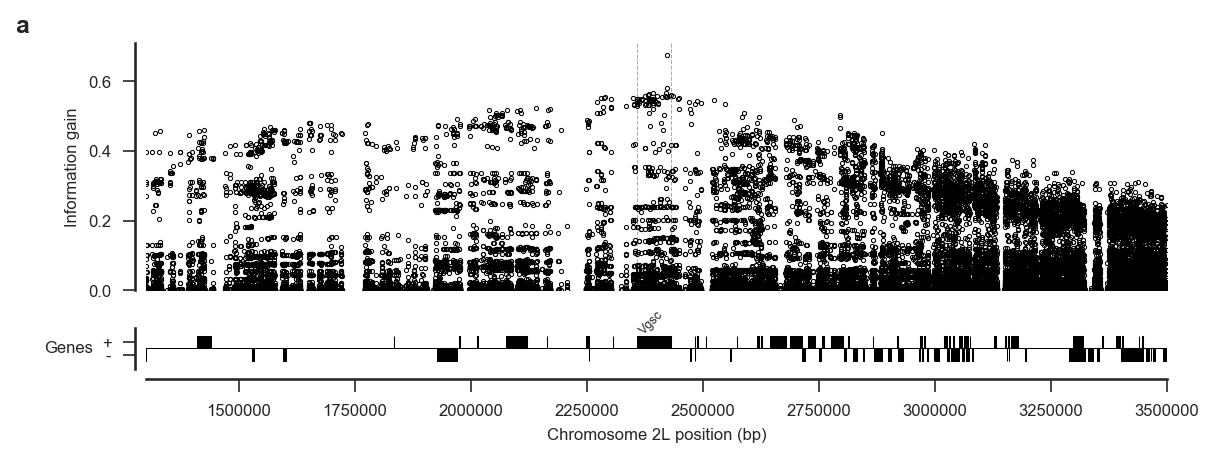
\includegraphics[width=1\linewidth,center]{artwork/chapter6/info_gain.png}
\end{subfigure}
\begin{subfigure}[t]{1\textwidth}
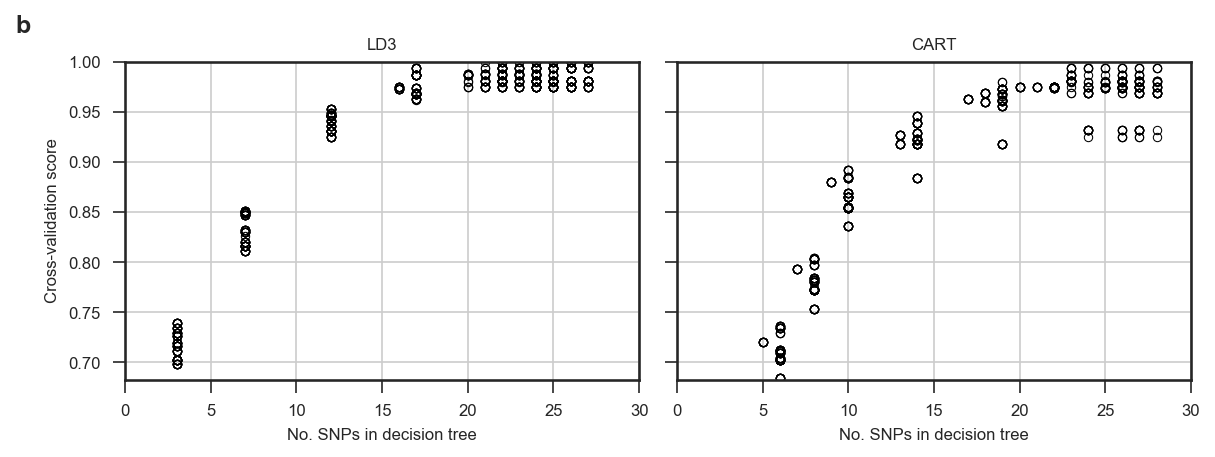
\includegraphics[width=1\linewidth,center]{artwork/chapter6/tree_cv.png}
\end{subfigure}
\caption{Ascertainment of informative SNPs for tracking resistance haplotypes.
%
\textbf{a}, Each data point represents a single SNP.
%
The information gain value for each SNP provides an indication of how informative the SNP is likely to be if used as part of a genetic assay for testing whether a mosquito carries a resistance haplotype, and if so, which haplotype group it belongs to.
%
\textbf{b}, Number of SNPs required to accurately predict which group a resistance haplotype belongs to.
%
Each data point represents a single decision tree.
%
Decision trees were constructed using either the LD3 (left) or CART (right) algorithm for comparison.
%
Accuracy was evaluated using 10-fold stratified cross-validation.
}
\label{fig:dt}
\end{figure}


To explore the feasibility of designing amplicon sequencing assays for tracking the spread of pyrethroid resistance, I investigated the minimum number of SNPs that would be required to differentiate the different resistance haplotype clusters discovered above.
%
I used the Ag1000G haplotype data to construct decision trees that could classify which of the haplotype clusters a given haplotype belongs to (Fig.~\ref{fig:dt}).
%
For each of two different tree-construction algorithms, I constructed decisions trees with a limit on the depth of the tree, repeating the process for progressively larger depths.
%
I then scored the classification performance of each tree via 10-fold stratified cross-validation.
%
These analyses suggested that it should be possible to classify haplotypes with $>95\%$ accuracy using a decision tree with 20 SNPs or less.
%
In practice, more SNPs would be needed to provide some redundancy, and also to type non-synonymous polymorphisms in addition to identifying the genetic background.
%
However, it is still likely to be well within the number of SNPs that could be assayed in a single amplicon sequencing multiplex.
%
Thus, it should be feasible to produce low-cost, high-throughput genetic assays for tracking the spread of pyrethroid resistance.
%
If combined with a limited amount of whole-genome sequencing at sentinel sites across a broad geographical range, this could also allow targeted assays to be continuously updated to track newly emerging resistance outbreaks.



%%%%%%%%%%%%%%%%%%%%%%%%%%%%%%%%%%%%%%%%%%%%%%%%%%%%%%%%%%%%%%%%%%%%%%%%%%%%%%%
%%%%%%%%%%%%%%%%%%%%%%%%%%%%%%%%%%%%%%%%%%%%%%%%%%%%%%%%%%%%%%%%%%%%%%%%%%%%%%%
%%%%%%%%%%%%%%%%%%%%%%%%%%%%%%%%%%%%%%%%%%%%%%%%%%%%%%%%%%%%%%%%%%%%%%%%%%%%%%%
\section{Conclusions}\label{sec:conclusions}


Molecular evolution of pyrethroid target-site resistance is clearly far more complex than previously appreciated.
%
Secondary evolution is occurring on haplotypes carrying the primary \texttt{L995F} allele, leading to double and triple mutant haplotypes.
%
The phenotype of these combined mutants needs to be urgently characterised, because \textit{Vgsc} combination mutants in other insect species have far higher levels of pyrethroid resistance than single mutants.
%
The operational significance of these mutants for malaria vector control also needs to be urgently characterised, to investigate any effect on ITN efficacy.
%
Resistance alleles are also clearly spreading between countries, in some cases reaching countries separated by up to 4,000 km.
%
This includes alleles spreading between countries on both sides of the equatorial rainforest, and on both sides of the East African Rift, which was surprising given the relatively high levels of genome-wide differentiation between these populations observed in Chapter 4.
%
Thus, the \textit{Vgsc} gene reveals how mosquito populations are connected across the continent, and how resistance alleles can spread even where rates of gene flow might otherwise appear low.
%
In the next and final chapter I discuss the implications of these and other findings from this thesis for the future of malaria vector control, and review both the opportunities and challenges involved in developing genomic surveillance systems for malaria vectors.


%%%%%%%%%%%%%%%%%%%%%%%%%%%%%%%%%%%%%%%%%%%%%%%%%%%%%%%%%%%%%%%%%%%%%%%%%%%%%%%
%%%%%%%%%%%%%%%%%%%%%%%%%%%%%%%%%%%%%%%%%%%%%%%%%%%%%%%%%%%%%%%%%%%%%%%%%%%%%%%
%%%%%%%%%%%%%%%%%%%%%%%%%%%%%%%%%%%%%%%%%%%%%%%%%%%%%%%%%%%%%%%%%%%%%%%%%%%%%%%
\section{Methods}\label{sec:methods}


%%%%%%%%%%%%%%%%%%%%%%%%%%%%%%%%%%%%%%%%%%%%%%%%%%%%%%%%%%%%%%%%%%%%%%%%%%%%%%%
%%%%%%%%%%%%%%%%%%%%%%%%%%%%%%%%%%%%%%%%%%%%%%%%%%%%%%%%%%%%%%%%%%%%%%%%%%%%%%%
\subsection{Ascertainment of non-synonymous SNPs within the \textit{Vgsc gene}}\label{subsec:methods-asc}


I extracted all single nucleotide polymorphisms (SNPs) within the \textit{Vgsc} gene from the Ag1000G phase 1 data resource, and annotated each SNP according to its effect on the protein coding sequence.
%
Within the gene, a total of 63 non-synonymous SNPs were found, of which 51 passed and 12 failed genome-wide quality filters (Chapter 3).
%
One of the SNPs that failed quality filters was the known \texttt{N1570Y} resistance variant, but genome-wide SNP filters were generally conservative, erring on the side of minimising the false discovery rate at the expense of some sensitivity.
%
Because any non-synonymous SNP in the \textit{Vgsc} gene could potentially cause an important phenotypic effect, I performed a manual examination of genome accessibility metrics within all coding regions of the gene (Fig.~\ref{fig:accessibility}).
%
All the non-synonymous SNPs within the gene that failed quality filters were close to the thresholds set, and there was no evidence of structural variation, alignment ambiguity or other accessibility issues in any of the gene exons.
%
I therefore included all 63 non-synonymous SNPs in subsequent analyses.


The Vgsc gene is also known to undergo splicing variation in multiple insect species including \agam, and this is believed to be an important factor enabling insects to achieve phenotypic variation in different tissues~\parencite{Dong2014,Davies2007}.
%
For \agam, at the time this analysis was performed, three transcripts were present in the AgamP4.4 gene annotations provided by VectorBase, which derived primarily from automated gene predictions~\parencite{Curwen2004}.
%
However, the canonical study of the \textit{Vgsc} gene in \agam\ is \textcite{Davies2007}, where substantially greater splice variation was reported.
%
A difficulty of the data from \textcite{Davies2007} is that there are no complete transcript sequences, only separate cDNA sequences from the first and second halves of the transcript.
%
To allow for all possibilities, I constructed a set of transcripts from all possible combinations of the first and second half cDNA sequences (Fig.~\ref{fig:transcripts}).
%
Some of these transcripts included optional exons or exon regions not represented in the VectorBase transcripts.
%
I then reran SNP effect predictions for all SNPs discovered within the Vgsc gene with each of these alternative transcripts, to determine whether any non-synonymous SNPs had occurred within an exon or exon segment not present in the canonical AgamP4.4 \texttt{AGAP004707-RA} transcript.
%
Three additional non-synonymous variants were found in these other transcripts, one in each of exons 2j, 3 and 20d, but none of these occurred at above 3\% allele frequency in any population, and so were not analysed further.


%%%%%%%%%%%%%%%%%%%%%%%%%%%%%%%%%%%%%%%%%%%%%%%%%%%%%%%%%%%%%%%%%%%%%%%%%%%%%%%
%%%%%%%%%%%%%%%%%%%%%%%%%%%%%%%%%%%%%%%%%%%%%%%%%%%%%%%%%%%%%%%%%%%%%%%%%%%%%%%
\subsection{Additional phasing}\label{subsec:methods-phasing}


The haplotype data from Ag1000G phase 1 only include biallelic SNPs passing all quality filters, and thus did not include \texttt{N1570Y} due to failing genome-wide filters, nor the multiallelic SNPs at positions 2L:2,391,228 and 2L:2,400,071.
%
To incorporate these additional SNPs into the analysis, I phased these SNPs onto the Ag1000G haplotype scaffold using MVNcall version 1.0.


%%%%%%%%%%%%%%%%%%%%%%%%%%%%%%%%%%%%%%%%%%%%%%%%%%%%%%%%%%%%%%%%%%%%%%%%%%%%%%%
%%%%%%%%%%%%%%%%%%%%%%%%%%%%%%%%%%%%%%%%%%%%%%%%%%%%%%%%%%%%%%%%%%%%%%%%%%%%%%%
\subsection{Haplotype clustering and gene flow analyses}\label{subsec:methods-hapclust}


Haplotypes spanning the \textit{Vgsc} gene (\texttt{AGAP004707}, 2L:2,358,158--2,431,617) were extracted from the genome-wide dataset.
%
I computed the Hamming distance between all pairs of haplotypes, then performed hierarchical clustering of haplotypes and visualised the results as a dendrogram.
%
These analyses were performed using SciPy version 0.16.1~\parencite{Virtanen2020}.
%
To identify haplotype clusters, I cut the dendrogram at a distance of 12 SNPs and studied the largest clusters carrying \texttt{L1014F/S} resistance alleles.
%
A non-zero cutting distance allows for a small number of SNP differences within each cluster, which is expected as new mutations begin to occur on haplotypes that are increasing in frequency under positive selection.
%
I used the complete linkage clustering method to generate the dendrogram and clusters reported here, but I repeated the analysis using the single and average linkage methods, finding highly concordant results.


To investigate whether recombination events within the \textit{Vgsc} gene might have affected the clustering of haplotypes carrying resistance alleles, I performed an additional analysis using data from regions flanking the gene.
%
I repeated the clustering analysis separately on non-overlapping windows upstream and downstream of the \textit{Vgsc} gene, using the same window size (1,718 SNPs) as used for the clustering analysis within the gene.
%
I then compared the resulting haplotype clusters by computing the set intersection between all pairs of clusters across all pairs of windows.
%
If recombination events happened, this would affect the haplotype clustering in some windows but not others, causing some discordance between clustering in adjacent windows.
%
In the window immediately upstream of the gene I found clusters with at least 93\% intersection with the clusters identified within the gene, except for clusters S4 and S5 which merged into a single cluster.
%
In the window immediately downstream of the gene I found clusters with at least 93\% intersection, again except for S4 and S5 which merged into a single cluster, and except for F1 which split into a major cluster carrying 402/465 (86\%) of the F1 cluster and a minor cluster carrying 60/465 haplotypes.
%
The most parsimonious explanation for the S4/S5 clustering together on both flanks of the gene is that these are both derived from the same haplotype, but experienced a gene conversion or sequence of crossover events within the \textit{Vgsc} gene to bring some portion of a different haplotype into the original genetic background.
%
The region of differentiation between S4 and S5 is limited to a 13 kb region upstream of codon 995, and these two clusters share haplotype homozygosity spanning codon 995.


To confirm evidence of resistance allele gene flow between populations, I performed a between-population analysis of haplotype homozygosity, implemented via a custom Python script.
%
Briefly, this analysis extracts haplotypes from each of two populations in moving windows of 2000 SNPs across chromosome arm 2L, and computes the fraction of haplotype pairs that are identical (haplotype homozygosity), considering only pairs with one haplotype from each population.
%
A value of 0 indicates no haplotype pairs are identical between populations, and a value of 1 indicates all haplotype pairs are identical between populations.


%%%%%%%%%%%%%%%%%%%%%%%%%%%%%%%%%%%%%%%%%%%%%%%%%%%%%%%%%%%%%%%%%%%%%%%%%%%%%%%
%%%%%%%%%%%%%%%%%%%%%%%%%%%%%%%%%%%%%%%%%%%%%%%%%%%%%%%%%%%%%%%%%%%%%%%%%%%%%%%
\subsection{Positive selection}\label{subsec:methods-selection}


Core haplotypes were defined on a 6,078 bp region spanning \textit{Vgsc} codon 995, from chromosome arm 2L position 2,420,443 and ending at position 2,426,521.
%
This region was chosen as it was the smallest region sufficient to differentiate between the ten haplotype clusters carrying either of the known resistance alleles L1014F or L1014S.
%
Extended haplotype homozygosity (EHH) was computed for all core haplotypes as described in \textcite{Sabeti2002} using scikit-allel version 1.1.9, excluding non-synonymous and singleton SNPs.


%%%%%%%%%%%%%%%%%%%%%%%%%%%%%%%%%%%%%%%%%%%%%%%%%%%%%%%%%%%%%%%%%%%%%%%%%%%%%%%
%%%%%%%%%%%%%%%%%%%%%%%%%%%%%%%%%%%%%%%%%%%%%%%%%%%%%%%%%%%%%%%%%%%%%%%%%%%%%%%
\subsection{Decision tree analyses}\label{subsec:methods-dts}


To explore the feasibility of identifying a small subset of SNPs that would be sufficient to identify each of the genetic backgrounds carrying known or putative resistance alleles, I started with an input data set of all SNPs within the \textit{Vgsc} gene or in the flanking regions 20 kbp upstream and downstream of the gene.
%
Each of the 1530 haplotypes in the Ag1000G phase 1 cohort was labelled according to which core haplotype it carried, combining all core haplotypes not carrying known or putative resistance alleles together as a single "wild-type" group.
%
Decision tree classifiers were then constructed using scikit-learn version 0.19.0 for a range of maximum depths, repeating the tree construction process 10 times for each maximum depth with a different initial random state.
%
The classification accuracy of each tree was evaluated using stratified 10-fold cross-validation.


\printbibliography


\clearpage
\beginsupplement
%%%%%%%%%%%%%%%%%%%%%%%%%%%%%%%%%%%%%%%%%%%%%%%%%%%%%%%%%%%%%%%%%%%%%%%%%%%%%%%
%%%%%%%%%%%%%%%%%%%%%%%%%%%%%%%%%%%%%%%%%%%%%%%%%%%%%%%%%%%%%%%%%%%%%%%%%%%%%%%
%%%%%%%%%%%%%%%%%%%%%%%%%%%%%%%%%%%%%%%%%%%%%%%%%%%%%%%%%%%%%%%%%%%%%%%%%%%%%%%
\section{Supplemental figures}\label{sec:supplemental-figures}


\clearpage
\begin{landscape}

\begin{figure}
\centering
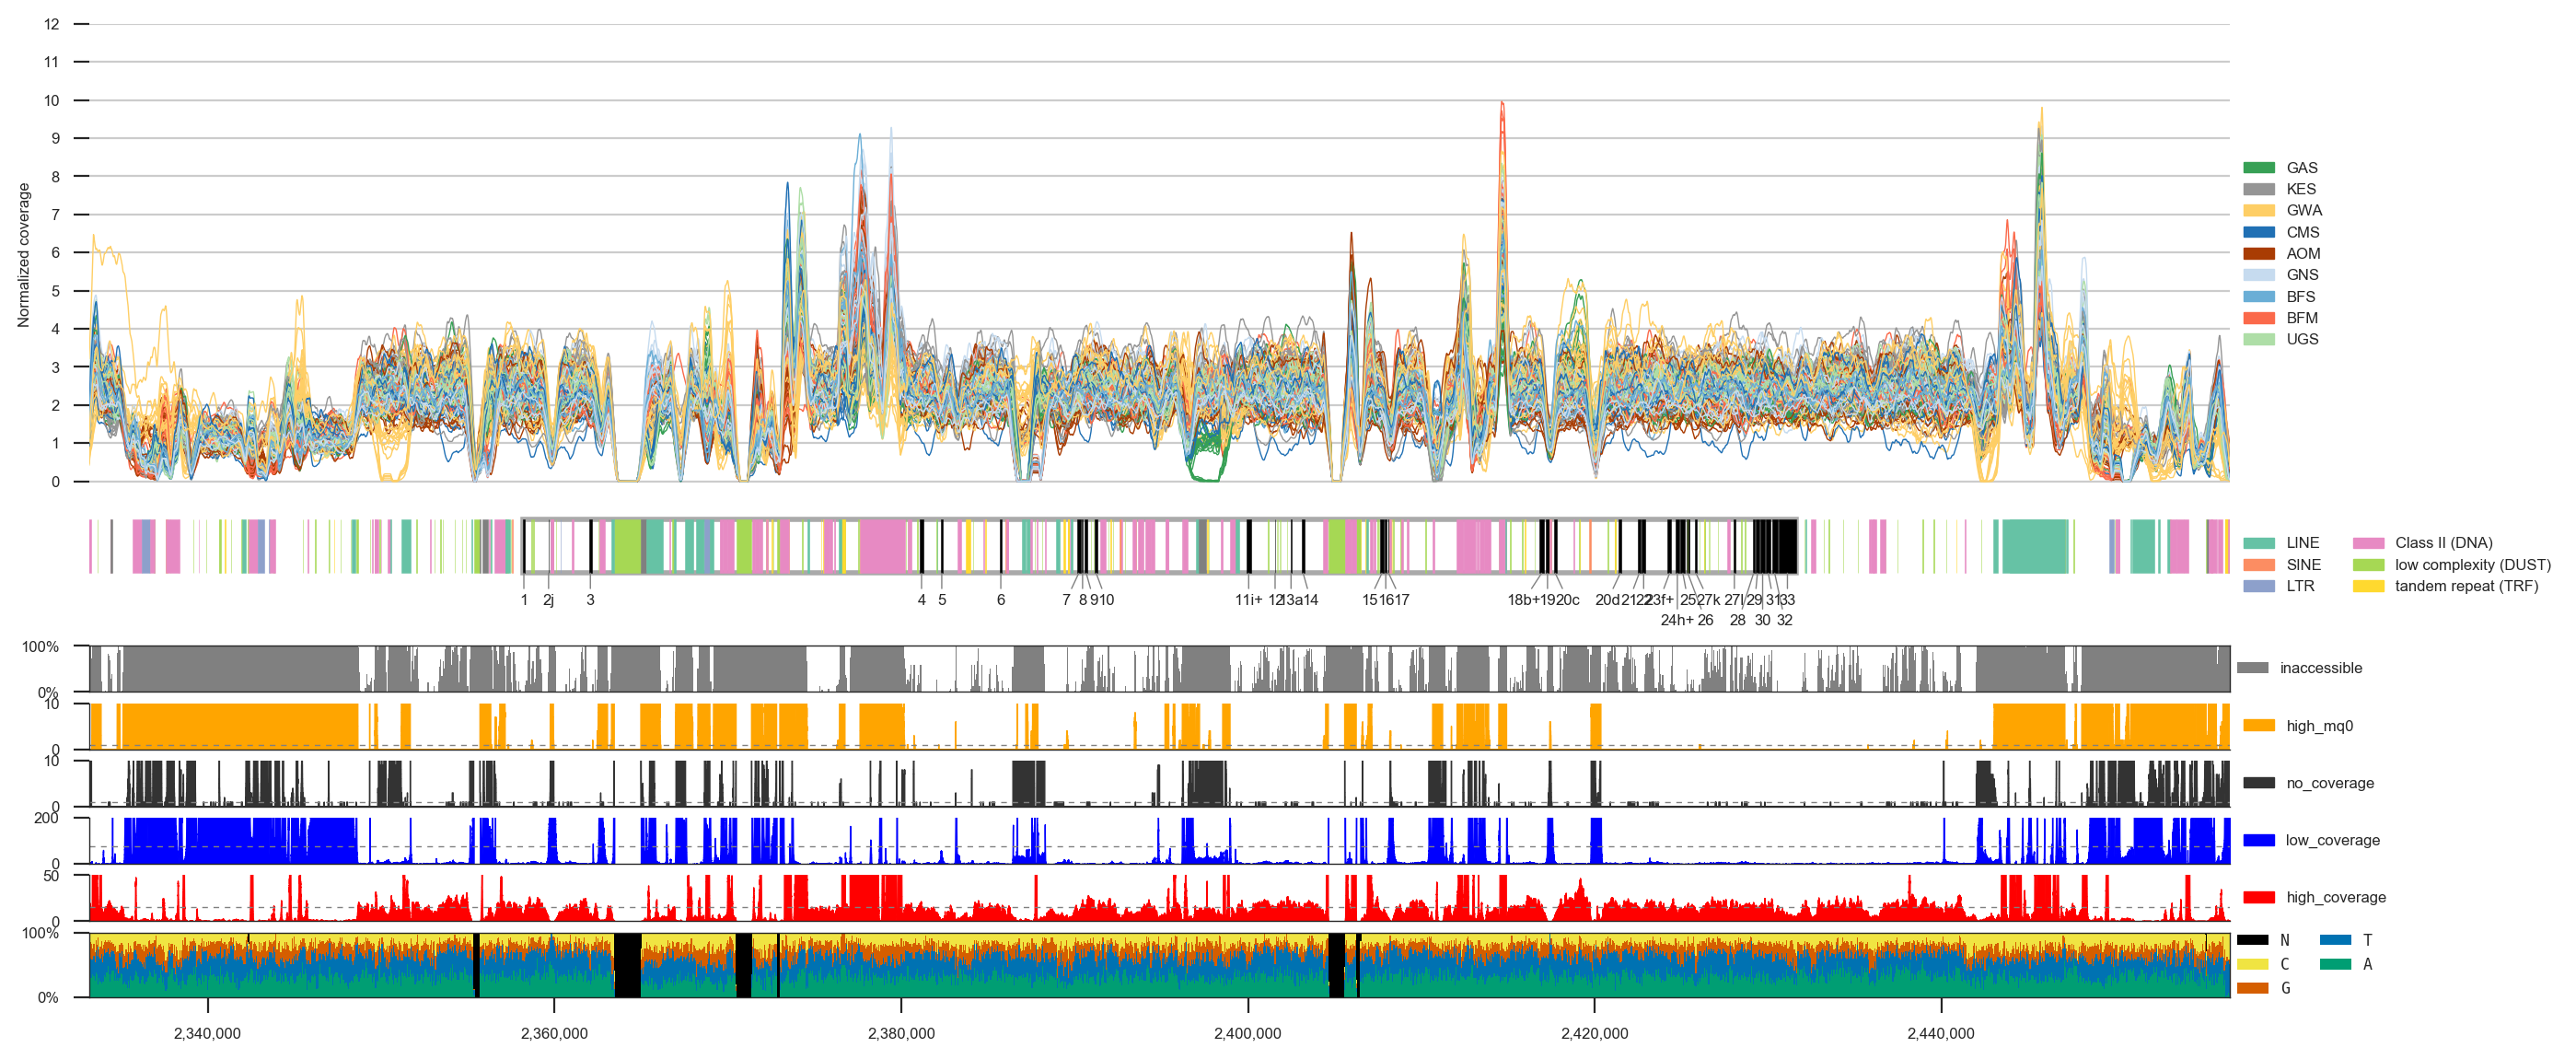
\includegraphics[width=1.1\linewidth,center]{artwork/chapter6/accessibility.png}
\caption{Accessibility of the \textit{Vgsc} gene.
%
Upper plot shows coverage traces for all individuals in the Ag1000G phase 1 cohort, coloured by population, normalised by genome-wide coverage.
%
Schematic below shows locations of \textit{Vgsc} gene exons (black) and different classes of repetitive or low complexity sequences.
%
Tracks at the bottom show plots of various genome accessibility metrics.
}
\label{fig:accessibility}
\end{figure}

\end{landscape}


\clearpage
\begin{landscape}

\begin{figure}
\centering
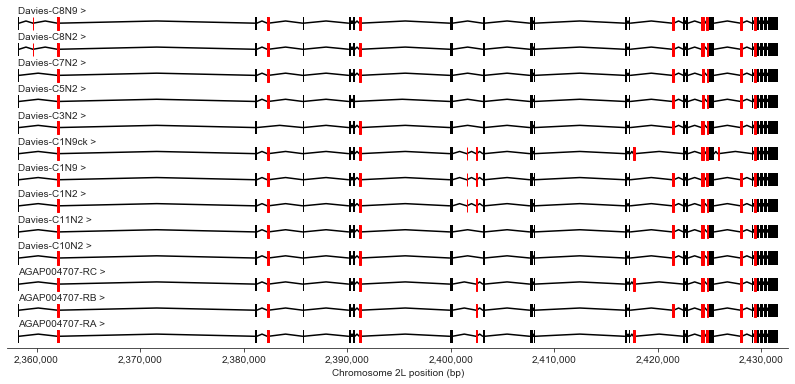
\includegraphics[width=0.8\linewidth,center]{artwork/chapter6/transcripts.png}
\caption{Alternative transcripts for the \textit{Vgsc} gene, inferred from cDNA sequences reported by \textcite{Davies2007}.
}
\label{fig:transcripts}
\end{figure}

\end{landscape}


\clearpage
\begin{figure}[t!]
\centering
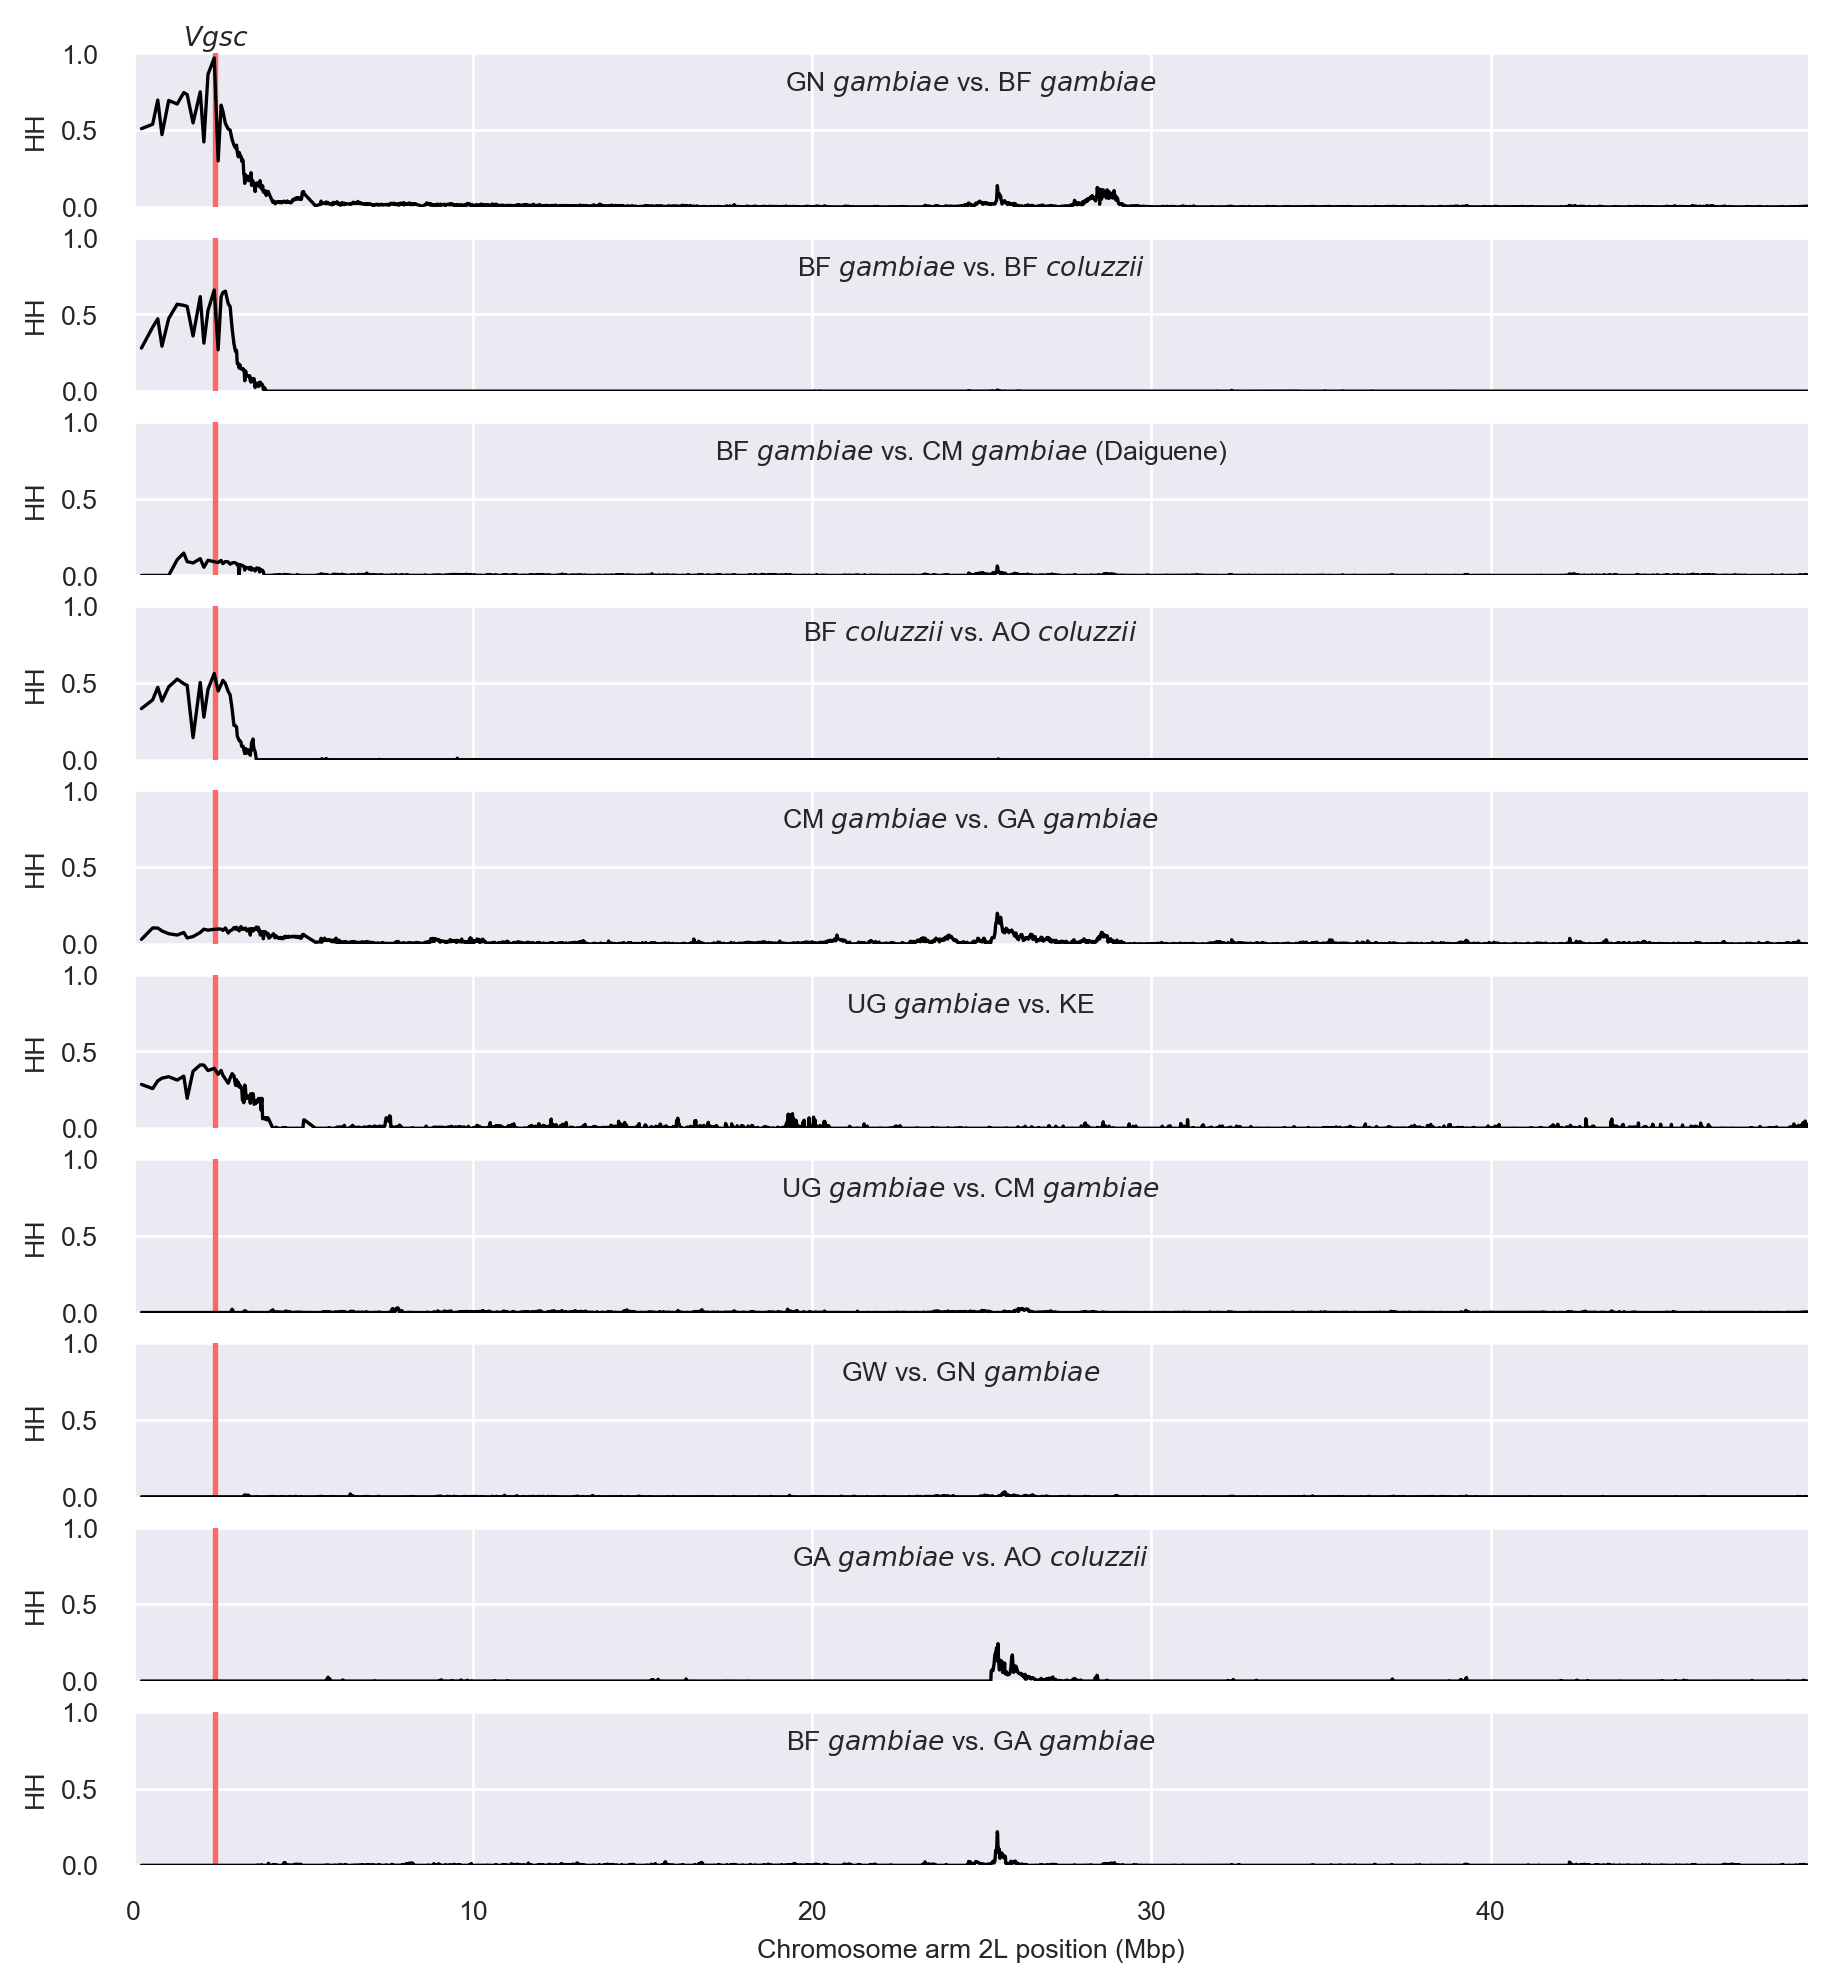
\includegraphics[width=1.1\linewidth,center]{artwork/chapter6/xphh.png}
\caption{Chromosome-wide scans for between-population haplotype homozygosity (HH).
%
Each track plots the fraction of between-population haplotype pairs that are identical within moving windows of 2,000 SNPs.
%
A value of 1 indicates all haplotype pairs are identical.
%
A value of 0 indicates no haplotype pairs are identical.
}
\label{fig:xphh}
\end{figure}


\clearpage
\begin{figure}[t!]
\centering
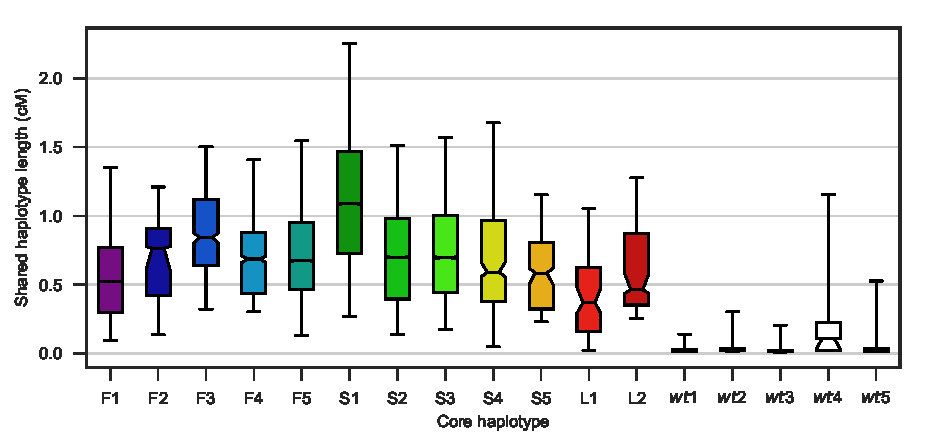
\includegraphics[width=1.1\linewidth,center]{artwork/chapter6/pspd.pdf}
\caption{Analysis of shared haplotype lengths.
%
Each bar shows the distribution of shared haplotype lengths between all pairs of haplotypes with the same core haplotype.
%
For each pair of haplotypes, the shared haplotype length was computed as the region extending upstream and downstream from the core locus (\textit{Vgsc} codon 995) over which haplotypes are identical at all non-singleton variants.
%
The \textit{Vgsc} gene sits on the border of pericentromeric heterochromatin and euchromatin, and I assumed different recombination rates in upstream and downstream regions.
%
The shared haplotype length is expressed in centiMorgans (cM) assuming a constant recombination rate of 2.0 cM/Mb on the downstream (euchromatin) flank and 0.6 cM/Mb on the upstream (heterochromatin) flank.
%
Bars show the inter-quartile range, fliers show the $5-95^{th}$ percentiles, horizontal black line shows the median, notch in bar shows the 95\% bootstrap confidence interval for the median.
%
Haplotypes F1--5 each carry the \texttt{L995F} resistance allele.
%
Haplotypes S1--5 each carry the \texttt{L995S} resistance allele.
%
Haplotype L1 carries the \texttt{I1527T} allele.
%
Haplotype L2 carries the \texttt{M490I} allele.
%
Wild-type (wt) haplotypes do not carry any known or putative resistance alleles.
}
\label{fig:pspd}
\end{figure}


\end{document}
